% !TeX program = xelatex
\documentclass[12pt]{article}

\usepackage{polyglossia}
\setmainlanguage{russian}
\setotherlanguage{english}

\setmainfont[
SmallCapsFont={Latin Modern Roman Caps},
SmallCapsFeatures={Letters=SmallCaps},
Ligatures=TeX
]{Times New Roman}

\usepackage[intlimits]{amsmath}
\usepackage{amssymb}
\usepackage{mathrsfs}
\usepackage{indentfirst}
\usepackage{graphicx}
\usepackage[margin=2cm]{geometry}

\newcommand{\pd}[2]{\frac{\partial #1}{\partial #2}}
\newcommand{\dpd}[2]{\dfrac{\partial #1}{\partial #2}}

\newcommand{\pdd}[2]{\frac{\partial^2 #1}{\partial #2^2}}
\newcommand{\pddd}[3]{\frac{\partial^2 #1}{\partial #2\partial #3}}

\renewcommand{\arraystretch}{1.2}
\let\dividesymbol\div
\renewcommand{\div}{\operatorname{div}}
\newcommand{\grad}{\operatorname{grad}}
\newcommand{\rot}{\operatorname{rot}}
\newcommand{\const}{\operatorname{const}}
\renewcommand{\vec}[1]{\boldsymbol{\mathbf{#1}}}
\newcommand{\ten}[1]{\mathbf{#1}}
\newcommand{\cutefrac}[2]{{}^{#1}\mkern-5mu/{\!}_#2}
\newcommand{\half}{{\cutefrac{1}{2}}}
\renewcommand{\leq}{\leqslant}
\renewcommand{\geq}{\geqslant}

\author{Цыбулин Иван}
\title{Осциллятор Ван-дер-Поля}
\date{}

\begin{document}
\maketitle

\emph{Данную задачу разбирали на лекции, привожу здесь краткое изложение.}

Уравнение Ван-дер-Поля в виде системы второго порядка имеет вид
\[
\begin{cases}
y_1' = \mu\left(y_1 - \frac{y_1^3}{3}\right) + y_2,\\
y_2' = -y_1
\end{cases}
\]
Здесь $\mu \gg 1$ --- параметр. 

\emph{Определить тип особой точки системы}. $(y_1, y_2)$ будет особой точкой системы если в ней выполняется $y_1'=0, y_2'=0$. В данном случае единственной особой точкой будет $(0, 0)$. В окрестности $(0, 0)$ система ведет себя как линейная
\[
\begin{cases}
y_1' = \mu y_1 + y_2,\\
y_2' = -y_1
\end{cases}
\]
Собственные числа матрицы 
$$
\begin{pmatrix}
\mu & 1\\
-1 & 0
\end{pmatrix}
$$
равны $\lambda = \frac{\mu \pm \sqrt{\mu^2 - 4}}{2}$. При $\mu > 2$ оба числа положительные, и особая точка имеет тип <<неустойчивый узел>>, при $0 < \mu < 2$ собственные числа комплексные, с положительной действительной частью, и особая точка имеет тип <<неустойчивый фокус>>. Таким образом, точка $(0, 0)$ --- неустойчивая.

\emph{Решение на фазовой плоскости}. Изучим поведение решения уравнения Ван-дер-Поля на фазовой плоскости $(y_1, y_2)$. Для этого полезно изобразить на ней линию, соответствующую
$y_1' = 0$. Условие $y_1' = 0$ задает кубическую параболу
\[
y_2 = \mu \left(\frac{y_1^3}{3} - y_1\right),
\]
траектории системы пересекают эту параболу вертикально ($y_1' = 0$) сверху вниз при $y_1 > 0$ и снизу вверх при $y_1 < 0$. Вершины параболы расположены в точках $(\mp 1, \pm \frac{2}{3}\mu)$.

Вдали от параболы траектории имеют вид практически горизонтальных участков, направленных вправо ($y_1' > 0$), если находятся выше параболы, и влево ($y_1' < 0$), если находятся ниже.

\begin{figure}[ht!]
\centering
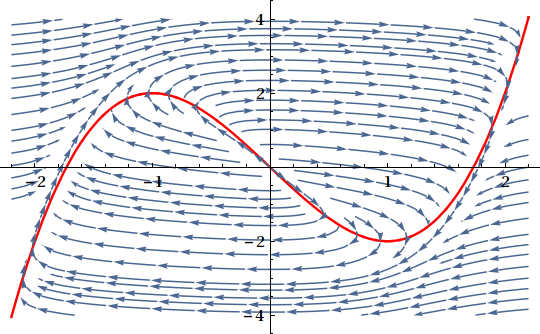
\includegraphics[width=.5\textwidth]{vdp.png}%
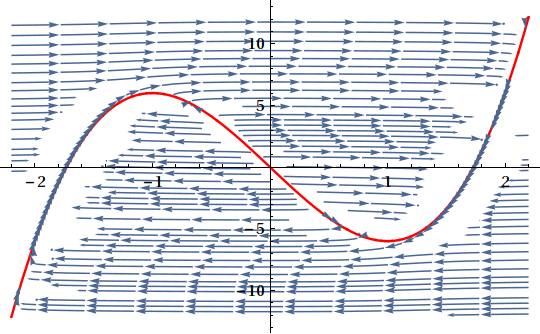
\includegraphics[width=.5\textwidth]{vdp9.png}%
\caption{Фазовая плоскость для $\mu = 3$ (слева) и $\mu = 9$ (справа)}
\end{figure}

Отметим, что приближаясь к параболе траектории решения круто поворачивают: вдали от параболы они движутся горизонтально, а параболу пересекают уже вертикально. Чем больше $\mu$, тем круче поворачивают траектории. Такое поведение траекторий говорит о жесткости задачи в этой области.

Изучим жесткость задачи алгебраически: найдем спектр матрицы Якоби правой части системы дифференциальных уравнений Ван-дер-Поля в зависимости от положения на фазовой плоскости.
\[
\vec J(y_1, y_2) = \pd{(y_1', y_2')}{(y_1, y_2)} = 
\begin{pmatrix}
\mu (1 - y_1^2) & 1\\
-1 & 0
\end{pmatrix}
\]
Найдем собственные числа матрицы Якоби $\vec J$:
\[
0 = \det (\vec J - \lambda \vec E) = (\lambda - \mu (1 - y_1^2) ) \lambda + 1 = 
\lambda^2 - \mu (1 - y_1^2) \lambda + 1
\]
\[
\lambda_{1,2} = \frac{\mu(1 - y_1^2) \pm \sqrt{\mu^2 (1 - y_1^2)^2 - 4}}{2}
\]
Из теоремы Виета сразу можем заключить, что $\lambda_1 \lambda_2 = 1$. Если $|\mu (1 - y_1^2)| \leq 2$, то корни уравнения комплексно сопряжены и оба лежат на единичной окружности:
\begin{figure}[ht!]
\centering
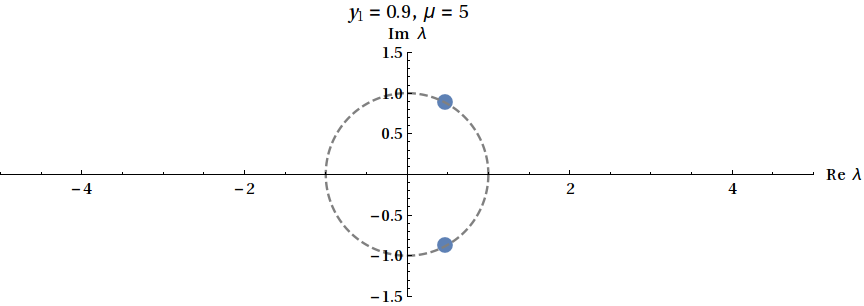
\includegraphics[width=\textwidth]{lamcc.png}
\end{figure}
Задача не является жесткой в этой области (спектр не распадается на жесткую и мягкую компоненты).

Рассмотрим оставшиеся два варианта:
\begin{itemize}
\item $\mu(1 - y_1^2) > 2 \Leftrightarrow y_1^2 < 1 - \frac{2}{\mu}$. В этом случае
\[
\lambda_{1,2} = \frac{\mu(1 - y_1^2) \pm \sqrt{\mu^2 (1 - y_1^2)^2 - 4}}{2} > 0,
\]
Оба собственных числа положительны. В этой части фазовой плоскости задача не является жесткой (в жесткой задаче жесткая компонента спектра должна лежать в левой полуплоскости), более точно задача в этой области фазовой плоскости является неустойчивой по Ляпунову.
\begin{figure}[ht!]
\centering
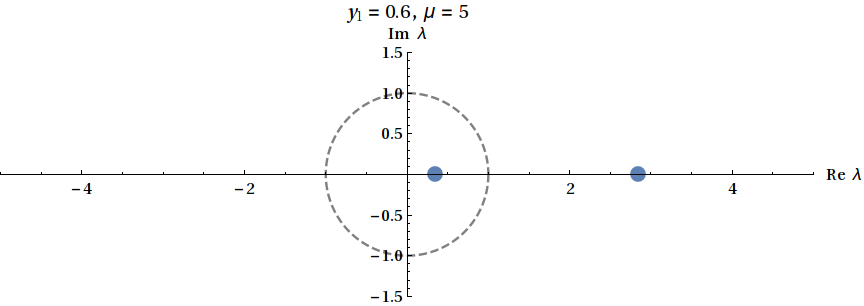
\includegraphics[width=\textwidth]{lamunst.png}
\end{figure}
\item $\mu(1 - y_1^2) < -2 \Leftrightarrow y_1^2 > 1 + \frac{2}{\mu}$. В этом случае
\[
\lambda_{1,2} = \frac{\mu(1 - y_1^2) \pm \sqrt{\mu^2 (1 - y_1^2)^2 - 4}}{2} < 0,
\]
Оба собственных числа отрицательны. В этой части фазовой плоскости задача является жесткой. \begin{figure}[ht!]
\centering
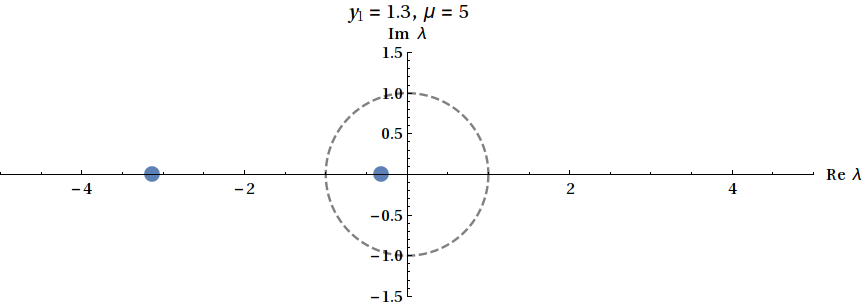
\includegraphics[width=\textwidth]{lamst.png}
\end{figure}
\end{itemize}
Показателем жесткости $\frac{L}{\ell}$ будет являться отношение собственных чисел $\lambda_1$ и $\lambda_2$ (считаем, что $\lambda_1$ --- жесткий спектр, $\lambda_2$ --- мягкий, то есть $\operatorname{Re} \lambda_1 = -L \ll -\ell = -|\lambda_2|$):
\[
\frac{L}{\ell} = \frac{\lambda_1}{\lambda_2} = 
\frac{\lambda_1}{1 / \lambda_1} = \lambda_1^2.
\]
Если принять $\mu (1 - y_1^2) \ll -2$, то выражение для $\lambda_1$ упрощается до
\[
\lambda_1 \approx \frac{\mu(1 - y_1^2) - |\mu(1 - y_1^2)|}{2} = \mu(1 - y_1^2),
\]
а для $\lambda_2$, соответственно,
\[
\lambda_2 = \frac{1}{\lambda_1} \approx \frac{1}{\mu(1 - y_1^2)}.
\]
Для показателя жесткости задачи получаем оценку
\[
\frac{L}{\ell} \approx \mu^2 (1 - y_1^2)^2
\]
в области жесткости $y_1^2 > 1 + \frac{2}{\mu}$.

Решение уравнения Ван-дер-Поля имеет предельный цикл. Это значит, что начиная из любой точки фазового пространства (кроме начала координат), решение будет стремиться к периодическому решению, изображенному ниже:
\begin{figure}[ht!]
\centering
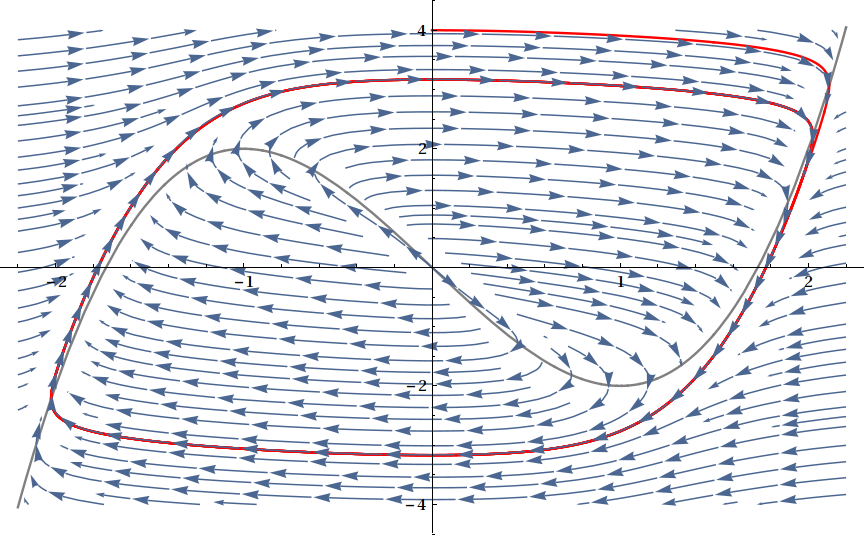
\includegraphics[width=\textwidth]{limit.png}
\caption{Решение системы из начальной точки $(0,4)$ быстро стремится к предельному циклу. Случай $\mu = 3$.}
\end{figure}

Таким образом, находясь вблизи предельного цикла, величина $(1 - y_1^2)^2$ не превышает существенно значения $(1 - y_1^2)^2 \approx 9$, то есть показатель жесткости задачи не превышает $9\mu^2$. При больших $\mu$ можно считать, что задача жесткая в области $|y_1| > 1$.

\end{document}